\chapter{Modellarchitektur und Ablauf}

Diese kleine Einleitung soll dem Nutzer helfen selbst die eigene Arbeit mit \LaTeX{} zu schreiben. Sie enthält zu den wichtigsten Themen Beispiele.


\section{2 Phasen der SER}

Für diese Arbeit lassen sich als Überschriften die Überschriften in verschiedenen Stufen verwenden.

\subsection{Verarbeitungseinheit (processing unit)}
\subsection{Klassifikator (classifier)}


\section{Aufbau der Modellarchitektur}


\begin{figure}[ht]
    \centering
    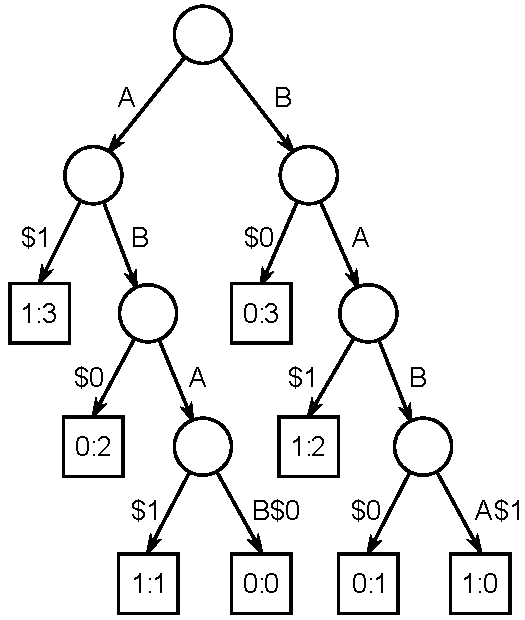
\includegraphics[width=.4\textwidth]{images/Suffix_tree_ABAB_BABA}
    \caption{\label{anker}Bechreibung des Bilds}
\end{figure}

Mit Hilfe eines Labels kann man sich dann im Text auf diese Grafik (\ref{anker}) beziehen. 

\begin{figure}[ht]
    \centering
    \subfigure[Ein fettes u]{
        
\includegraphics[width=0.2\linewidth]{images/a}
        \label{subfigurebsp:a}
    }
    \hspace{1cm}
    \subfigure[Ein dünneres u]{
        
\includegraphics[width=0.2\linewidth]{images/b}
        \label{subfigurebsp:b}
    }
    \caption{Die \emph{u}s aus der Wortmarke}
\end{figure}

Durch \verb|subfigure| lassen sich auch zwei kleine Bilder nebeneinander setzen. In Abbildung \ref{subfigurebsp:a} ist ein fettes u auf der linken und in \ref{subfigurebsp:b} ein dünneres auf der rechten Seite zu sehen.


\section{Der Ablauf bei SER}

Hier nur ein kurzes Beispiel, in jedem \LaTeX{} Buch finden sich gute Anleitungen zum Erstellen von Tabellen.





